% --------------------------------------------------------------------------- %
%      _ _                        _
%   __| (_)___  ___ _   _ ___ ___(_) ___  _ __
%  / _` | / __|/ __| | | / __/ __| |/ _ \| '_ \
% | (_| | \__ \ (__| |_| \__ \__ \ | (_) | | | |
%  \__,_|_|___/\___|\__,_|___/___/_|\___/|_| |_|
% --------------------------------------------------------------------------- %
\chapter{Implications for the Sonic Medium}
\label{sec: discussion}
\epigraph{\emph{Alice has stepped through the looking glass [...] It is the job all future artists and activists to use this technology for the better, to bring people together, and uproot social injustice.}}{\citep[]{skwarek2018}}

\begin{figure}
    \centering
    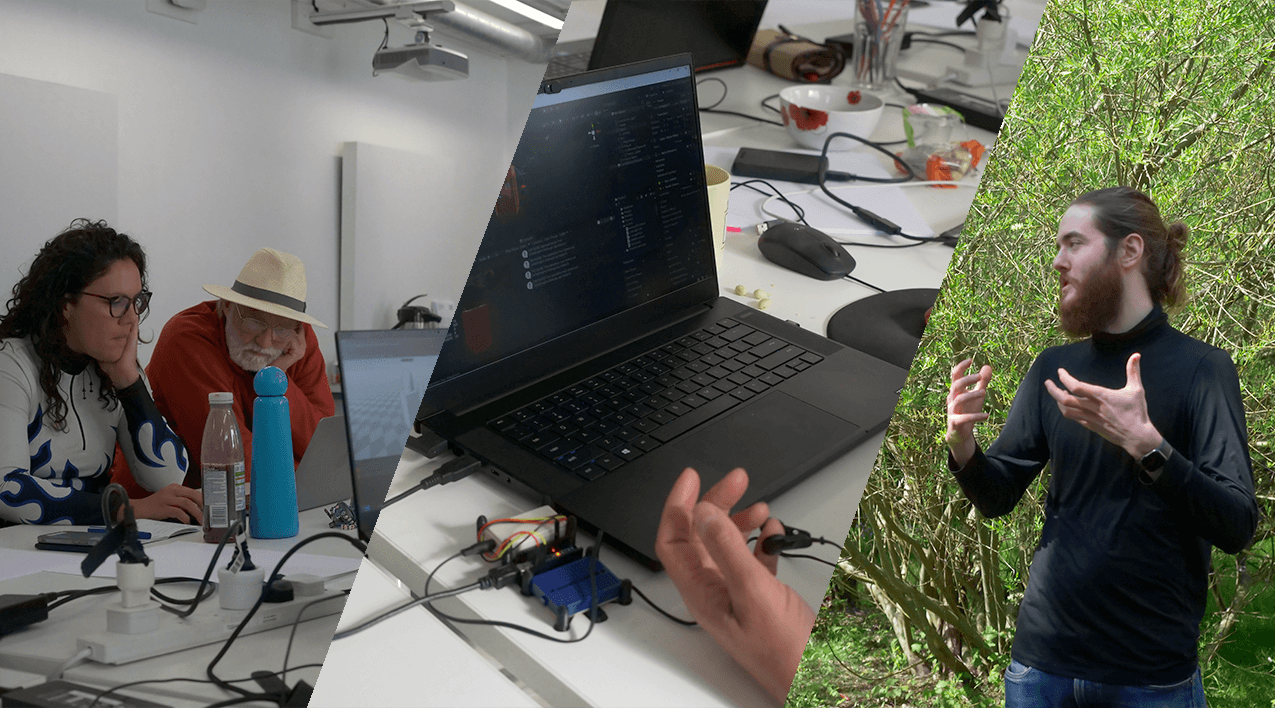
\includegraphics[width=1\linewidth]{08-discussion/chapter-fig.png}
    \captionsetup{labelformat=empty}
    \caption[Participants experiencing and demonstrating usage of Project North Star (own photographs)]{}
\end{figure}

\clearpage
% --------------------------------------------------------------------------- %
\section{Summary}\label{sec: discussion-summary}
In this chapter I aim to bring together the results of the past three study chapters, and discuss the implications they may have on what could be termed the sonic medium of \gls{ar}. It is separated into three sections. In the first, I review the steps taken so far in the thesis that have allowed space for a unique positionality when considering the potential for \gls{ar} as a medium for sound-driven art works. In the second, I outline the methodology that lead to the sound \gls{art} that makes up my practice-based research. In the third section, the combined results of the previous three chapters are discussed in the context of materiality, embodiment, and space; resurfacing and re-introducing the theories explored in \autoref{sec: theory}.
% --------------------------------------------------------------------------- %
\section{From Overlay to Instrument}\label{sec: discussion-review}
In \autoref{sec: introduction}, I outlined my motivations for asking the following questions, which were addressed in \autoref{sec: review} and \autoref{sec: theory}: 

\begin{itemize}
    \RQgenealogy
    \RQtheory
\end{itemize}

the present thesis began in \autoref{sec: review} with an exploration of the landscape of historical and contemporary \gls{ar} research and development spanning the past thirty years. Common forms, such as headset-, handheld- and projective-based \gls{ar} were outlined, as well as typical sensory displays, allowing interaction and feedback with the visual, auditory, touch-based, and smell and taste senses. Furthermore, the processes by which \gls{ar} mediates reality were laid out using Schraffenberger's categorisation of relationships and \gls{ar} subforms: augmented, diminished, altered, and hybrid reality, as well as extended perception \citep{schraffenberger2018}. Despite this wealth of possible avenues for \gls{ar} experience composition, the paradigmatic form of \gls{ar} we hear about or see are predominantly characterised by being \textit{visual displays that overlay information}. Thus far in the thesis, this has been referred to as ocularcentric layering paradigm, or typical \gls{ar}. This can be explained by a number of phenomena, but examining the origination of \gls{ar} in the \gls{mic} by way of U.S. Defence funding, it is not a surprise. This has had a compounded effect on the forms that \gls{ar} finds itself being co-opted for in the arts. Several creative and expressive works were explored, that engaged in \gls{ar} because of its ability to sensorily engage participants, induce rich aesthetic experience, enable collaborative expression, and empower new forms of agency and activism. Nonetheless, there are but a few examples of sound art \gls{ar} experiences in comparison to visual counterparts because of the typical form of \gls{ar}.

In proposing the development of \gls{ar} as a medium for the creation of immersive sound artworks, its use as an instrument, or tool for sound art installation, I drew on several areas of importance in \autoref{sec: theory}, first aesthetic experience and the `4E's', and then materiality, embodiment, and space. It began with a grounding in the concept of 'art as experience', drawing from the work of \citep{dewey1934}. Dewey states that the capitalistic reverence of fine art, notably by the `nouveau riches', has led to art being put on a pedestal - disconnecting it from its origin and operation in the everyday experiences of people. Leddy and Puolakka have since proposed that `material of art should be from all sources and art should be accessible to all' \citeyearpar{leddy2021}. Dewey points towards the aesthetic experience that art entails, and notes that the `live creature' is inseparable from the environment in which they are embedded. Today, despite social media as a platform for cultural production of artistic works has some merits, the fabric on which it is built is no different from the capitalist mechanisms that separated art from experience in the first place. Thus, \glshyperlink[open-source]{opensource}, hacker, \gls{diy}, and maker approaches were proposed as a method of democratising `all sources' of art, and attempting to increase accessibility. The focus on the body by Dewey also points towards the move towards tangible interface development, participatory design, and human-centred design that were outlined in \autoref{sec: method-resistance-maker}. To delve deeper into this experience of art, I proposed an enactivist approach to considering cognition in experience. Often called \gls{4ec}, it states that cognitive process are embodied, embedded, enactive, and extended \citep{gallagher2017}. In considering the design, performance, and experience of \gls{ar}, \gls{4ec} offers a fresh perspective on concepts such as agency, action, perception, immersion, and spatial engagement.

The first theoretical lens through which to examine \gls{ar}'s design in computational art and music practice involved outlined the importance of a complex systems framing of interface use and performance. I drew on existing research from the field of digital musical instrument design \citep{magnusson2009a,discipio2003,essl2006,armstrong2006,hayes2019,chevalier2018} in order to demonstrate the usefulness of considering the material of performance systems as complex, and ecosystemic. To examine what happens in the experience of participants, the second lens was one that took seriously the assertions of \gls{4ec}, namely that cognitive processes in experience are embodied, embedded, enactive and extended. I draw from multiple disciplines of similar theoretical and practical work in \gls{vr} and \gls{ar} to show how \gls{4ec} offers a novel framing by which to consider the experience of \gls{ar} by participants, audiences, and performers. Closing out the trio of theoretical lenses, is a grounding of the aforementioned consequence of \gls{ar} for the experience and construction of `space'. I first critically examine the term `Metaverse' \citep{stephenson1992}. Its modern-day origin is in technologies like \gls{ar} and \gls{vr}, which in turn sprung from` deep within the military and Western - scientific - industrial - patriarchal complex' \citep{davies2004}, and its current operation has been heavily co-opted by cryptocurrency projects. Because of this, in its current state, the `Metaverse' is hardly fertile ground for the `live creature' to experience art `accessibly', and from `all sources' \citep{dewey1934,leddy2021}, indeed, it mirrors the exact profit and exploitation motive of the historical context it originated in.



% --------------------------------------------------------------------------- %
\section{Engaging in a DIY Approach to Sound ARt}\label{sec: discussion-method}
A clear positionality from within the arts, one that stands in contrast with the militaristic and industrial applications and their effect on the typical form of \gls{ar} technologies was outlined in \autoref{sec: method}. This chapter proposed methodological approach to compose, iterate, and perform sound \gls{art} that would allow the addressing of the following research questions through practical contributions to the field of interactive music systems: 

\begin{enumerate}
    \RQmedium
    \RQexperience
    \RQfuture
\end{enumerate}

This began with the explication of the concept of resistance, and its importance in my rationale for choosing specific methods. Specifically, I highlighted the role of \gls{ar}'s paradigmatic form as a closed-source consumer technology, as a visual technology, and, and as a medium that overlays information, as primary motivators and areas for change in the field. In practice, this approach led to the evaluation of three aesthetically, functionally, and methodologically distinct interactive music systems over the course of the thesis, \textit{\nameref{sec: area} (2020)}, \textit{\nameref{sec: polaris} (2021)}, and \textit{\nameref{sec: polygons} (2022)}. These experiences, or sound \gls{art}works were developed using a set of design guidelines that were iterated on over the course of the thesis, and will be outlined in \autoref{sec: discussion-guidelines}. 

There are clear limitations to the the generalisability of specific findings in the \gls{ar} experiences developed. Having to adapt to the COVID-19 pandemic meant developing methods that revolved more around autoethnographic / autobiographical study of the systems. This, while potentially offering more depth of insight over long-term deployment of \textit{area\textasciitilde{}} for example, don't provide the kind of breadth of insight that the participant studies in \textit{polaris\textasciitilde{}} did for example. Qualitative analysis, while conducted with rigour throughout the thesis, still only speaks from a position that highlights the subjectivity of participant experience, and specificities of the experience being examined. There are, as always, positives and negatives to this. While providing considerable retrospective insight into my own creative practice, and providing the groundwork for developing the theoretical propositions in the next section, and patterns in \autoref{sec: discussion-guidelines}: \nameref{sec: discussion-guidelines}, they do not provide any objective and generalisable results about the nature of experience or reality. Perhaps there is no such thing, and the immense diversity of possible \gls{ar} experience serves to demonstrate this. Another benefit of the research methods involved in this approach is their propensity to provoke and generate questions, which have surfaced throughout this thesis.



% --------------------------------------------------------------------------- %
\section{Examining Sound ARt Experiences}\label{sec: discussion-medium}
\subsection{Combined Results: \textit{area\textasciitilde{}}, \textit{polaris\textasciitilde{}}, and \textit{polygons\textasciitilde{}}}
The previous three chapters outlined the experiences, compositions, performances, and results of engaging with \gls{ar} as a medium for sound \gls{art} production. In this section I would like to briefly touch on the findings from each.

\subsubsection{\textit{area\textasciitilde{}}}
\textit{area\textasciitilde{}}, which could be classified as a pilot study, or a research probe into the possibilities of non-visual \gls{ar} experience, uncovered the following results from an \gls{abd} research method. Firstly that the blending of \textit{real and virtual auditory environments} resulted aesthetically in the creation of a third, augmented environment that was greater in experiential nature than the sum of its parts (not simply a combinatorial layering). Secondly, the ability to spectromorphologically manipulate sounds in real-time in this augmented environment with the body proved an engaging compositional tool. Lastly, the potential for creating believable illusions of real-world sound sources from these manipulated and spatialised virtual sounds was highlighted.

\subsubsection{\textit{polaris\textasciitilde{}}}
\textit{polaris\textasciitilde{}}, through the evaluation of participant studies, and use of the grounded theory analysis method, found that \gls{av} \gls{ar} experiences are able to elicit a wide variety of emotions, and to explain and make sense of them participants often made use of metaphors and past experiences. Learning was one of the categories participants described, and it was clear that participants sensed this from multiple aspects of the experience, with one pointing towards the dimensionality, and others pointing towards the interactive elements and the need to explore the scene. In terms of adoption and comfortability, the fact that the headset lacked a good fit for most participants was clearly what detracted from the experience most. It led not only to a reduction in experience immersion, but also to a lessening of comfort and the knock-on effect of muscle fatigue and inability to exercise full agency for some participants. From the comments on different potential applications for \gls{ar}, it is clear that the offer of deeper interaction with subject matter, increased immersion in an experience, and the sense of \textit{`feeling'} or \textit{`playing'} with virtual content has led to participants envisaging \gls{ar}'s utilisation in several artistic and musical contexts. 

Control and self-expression was among the most highlighted categories, participants appreciated the ability to interact with their bare hands, and felt that this was the main contributor to their expression in the scene. This, for some, led to a feeling of power, and for some, a feeling of control over elements of the scene. For others, the feeling of control wasn't entirely certain, with some noting that the scene had agency of its own. It is also conclusive from these codes that some participants desired more control over the scene, although implementing this would have to be done thoughtfully, without overloading the scene with content and parameters to change.

Immersion tended to stem from the fact that the elements of the experience: sights, sounds, and actions were spatialised in three dimensions. Participants enjoyed and felt immersed by the movement and colour of the visual elements and were able to discern and localise the source of different sounds in the experience; several noting that this element was the most immersive factor for them, whilst others preferred the visual elements. Others still, noted that the actions that they employed, gestural and movement-based are what immersed them in the experience most, and for some, this led to the virtual content of the scene feeling physical at times.

\subsubsection{\textit{polygons\textasciitilde{}}}
\textit{polygons\textasciitilde{}}, the last of the experiences, could be described as a first look (or listen) into the implications of sound \gls{art} performances. For me, it provided a new, visceral type of embodied performance and led to a kind of `technologically mediated dialogue between hybrid self and hybrid environment', which in itself demonstrated the delicate balance of technological agency and sense of `uncontrol'. It provided me with the resulting questions: 
\begin{itemize}
    \item Can we avoid `spectacle' of \gls{ar}? How else can we meaningfully engage audiences who are new to \gls{ar}?
    \item How can we invite the audience into \gls{ar} musical performance more effectively?
    \item Is wearing more technology necessarily the best avenue for a focus on embodied performance?
    \item What would an \gls{ar} ensemble look, sound, and feel like for both performer and audience?
    \item Could \gls{ar} be appropriated for real-time networked performance of physically separate spaces?
\end{itemize}




\subsection[Augmented Materiality]{Augmented Materiality: The Relational Fabric of the AR(tistic) Medium}\label{sec: discussion-medium-material}
Core to my own approach is, as I'm sure is evident by now, is the centring of the notion of the processual nature of \gls{ar} systems. Ocularcentrism and the additive layering paradigm have shifted discussion of \gls{ar} systems towards an object-centred view of the `reality' that they present, this effect is also present in \gls{vr} \citep[]{hovhannisyan2019}. In \textit{\nameref{sec: area}}, \textit{\nameref{sec: polaris}}, and \textit{\nameref{sec: polygons}}, it was demonstrated that an \gls{ar} object is not a static visual thing with marked boundaries, not in any meaningful way to the artist/designer at least. It ought rather to be thought of as an on-going and distributed component existing inside a dynamic web of experience and meaning; and as such, any discussion of the contents or material of an \gls{ar} composition ought to be considered through this lens. Even a single apparent `virtual object' that is in front of a participant is not \textit{just} that; it is an invitation, a handle, a real-time process by which a participant can be perceptually guided through sensorimotor action towards a specific aesthetic experience. This so called `object' might be part of a larger organised whole, a component of a room-scale musical experience for example, or an emergent property of a hidden set of complex conditions that have only just been met through the specific movements of a participants body. This, more holistic, view of \gls{ar} processes allows for a more fruitful discussion of the types of experiences we can expect to craft as \gls{ar} practitioners; and engages more critically with Schraffenberger's taxonomy of \gls{ar} relationships.

Embedding Schraffenberger's fundamental relationships (\autoref{table:schraffenbergertaxonomy2}) within Di Scipio's notion of an `ecosystemic' musical interface, or Water's `performance ecosystem`, as outlined in \autoref{sec: theory-materiality}, could consist in viewing the \gls{ar} process as a real-time network of interactions distributed across the `hybrid' brain - body - environment. This helps us in identifying the \textit{medium specificity} of \gls{ar}, and how it may uniquely be deployed to create meaningful sound \gls{art}. If the motive for the composition of an artwork is to intentionally impart knowledge, meaning, or truth through aesthetic experience these must exist within and across the above network of interactions and relationships in our brain - body - environment distribution. I suggest that for the time being, we view this latent aesthetic experience as an real-time interaction between the components of:
\begin{itemize}
    \item Intention - the intended meaning behind the composition of the piece
    \item Medium - the specificity of the apparatus by which this meaning is imparted
    \item Experience - the on-going process by which the medium is engaged with by the participant
    \item Realisation - the resultant knowledge, truth, or subjective experience from of the above
\end{itemize}

\begin{table}
    \centering
    \begin{tabular}{ l l }
        \toprule
        Relationship        & Description                       \\
        \midrule
        Coexistence         & Unrelated                         \\
        Presence            & Spatially Related                 \\
        Information         & Content-Based Relationship        \\
        Physical            & Affect Each Other                 \\
        Behavioural         & Sense and React to Each Other     \\
        \bottomrule
    \end{tabular}
    \caption{Schraffenberger's Fundamental Relationships}\label{table:schraffenbergertaxonomy2}
\end{table}
In \autoref{sec: theory-experience}, we proposed that from Dewey's perspective, an artwork ought also to originate and operate within everyday sociocultural life in order to bring about positive social change through aesthetic experience. These concerns could be conceived as mainly arising from the component of intention, and its dynamic interaction through the medium into experience. Concerning the physical, or indeed virtual, manifestation of these intentions is that of the material composition - which is facilitated by the medium and its materiality. Of course, a consideration of the composition of a work cannot be divorced from the real-time experience of a participant, but from the perspective of the artist wanting to engage in these tools, an understanding of the inherent nature of the medium of \gls{ar} is necessary. Realisation of specific messages in the experience of artistic works could manifest in various ways, but one could argue that `the aesthetic experience' of the artwork has the potential to incur a feedback loop in which the participant is in a constant state of realisation, due to the nested, non-linear, and explorative aspects of the instrument or experience - drawing from Armstrong's realisational versus functional interface \citeyearpar{armstrong2006}. Perhaps they even come away from the artwork, imparted with changed beliefs or outlooks on the content of the experience; and then go on to act on these beliefs within their sociocultural life, thus leading to others potentially changing their own beliefs too.

In relation to the above constituent parts, in the context of Schraffenberger's relationships, what defines \gls{ar}'s medium specificity when chosen for the creation of expressive works of art, and how can these relations provide fertile ground for a new aesthetic of composition? The key element of these relations I argue, is the underlying assertion that what makes \gls{ar} unique is its ability to modulate the perceived conceptual 'distance' between real and virtual elements in three-dimensions and in real time. In Azuma's \citeyearpar[]{azuma1997} original definition of \gls{ar}, this is referred to as the `registration' or `alignment' of virtual content to real world content. I argue that Schraffenberger's fundamental relationships expand this concept beyond just a spatial alignment of elements. Presence-based relationships modulate this spatial distance between elements, while Information-based relationships modulate the thematic distance, Physical relationships modulate the material distance, and Behaviour-based relationships modulate the ecological distance. 

The narrative around the modulation of these various conceptual distances between real and virtual processes inevitably tends towards the closing of the gap between them. After all, the industries developing \gls{ar} view this as the `issue' of registration - the virtual and the real must be brought closer together. A U.S. marine wearing an \gls{ar} headset that provides him with a psychedelic experience of the true interconnectedness of all of reality, by exposing the incongruencies in our sensory stimuli through multisensory artwork that exploits and widens these conceptual distances, is a sure-fire way of Microsoft not being awarded any U.S. Army contracts in the future.

For a slightly more technological example, the resolution and acuity of motion and tracking sensors, normally viewed with the purpose of achieving an \gls{ar} that is spatially aligned to the perceived reality of the physical environment of the participant - thus closing the spatial distance through a Presence-based relationship between that `virtual object' and the physical environment. Another example might be an audio-tour. In this example, an Information-based relationship is invoked by closing the 'thematic distance' between virtual and real components, here, an abstract informational audio script becomes embedded in the actual environmental content of its real world setting. Schraffenberger argues that real and virtual objects casting shadows on each other constitutes a physical relationship - I'd argue that it is key to also view it as a reduction in the perceived material distance between the two objects (the way in which their physical matter behaves in respect to each other converges on the expected outcome of if both objects were physically real). Also proposed is that a virtual animal reacting to real world sounds would constitute a behavioural relationship - as you might expect, I'd argue that it must also be viewed as constituting a reduction in the perceived ecological distance between the animal and the sound (the set of behaviours that constitutes the interrelation of both environments converge on the outcome that would be expected if both animal and sound were members of our physical reality). These discussions of what I term 'closing the gap' usually fall under the banner of the drive for `increased immersion' or `believability'. 

However, just as \gls{ar} is demonstrated to be able to close the spatial, thematic, material, and ecological distance between the virtual and the real, so too can it further the gap between them. This is what Schraffenberger encapsulates in her argument for the proposal of the `relationship between the real and the virtual' to replace the proposal of the `registration of the virtual to the real' by Azuma among others. What if the thematic distance between the real and virtual is radically increased, but all others are kept the same? Could this be exploited for aesthetic effect? For artists using \gls{ar}, this is an important consideration — along with their definition of `real': is it synonymous with `truthful', `physical', `tangible'? What is the resultant aesthetic experience of participants if the virtual content of the artistic or musical \gls{ar} scene is divorced from the expectation of how a physical counterpart engages with space, theme, matter, and ecology? What about when going beyond representations or remediations of existing physical objects and processes, and presenting participants with radically novel virtual processes that still seem to be `embedded' in our physical reality via these technologies?

From this line of reasoning, the medium specificity of \gls{ar} could be said to be its `invocation of a performance ecosystem constituted of relationships between real and virtual processes in the axes of spatial, thematic, material and ecological distance'. If these relations are in turn experienced by a participant whose cognitive processes are embodied, embedded, enacted, and extended, it may stand to reason that the closer the distance between physical and virtual elements on these axes, the less discernible `physicality' and `virtuality' may become, and the cloudier the boundary between them. Despite being slightly alarming, this isn't to make the argument that a `virtual piano' might ever be mistaken for a `physical piano`, but I believe that the claim could be made that given enough time, a participants notion of what is `real about a piano' has the potential to be modulated, given that the virtual piano is at some level altered to be incongruous with its physical counterpart, but on most axes indiscernible from it. Perhaps it may look the same, but behaves differently, e.g. the keys play from high to low when pressed right to left. In this way, for a participant, the meaning and concept of a piano could change through this broader process of sensory or perceptual illusion, and then have real consequences in the physical world. This is a fairly benign example compared to what may be possible with future \gls{ar} technologies, and I view this as an important consideration for artists to hold: what are the ethical considerations I need to make as an artist who is using technologies that enable experiences such as this? What platforms am I using, and is telemetry gathered for a corporation of the technology that I am using? If \gls{ar} experiences are asking participants to suspend their disbelief in exchange for new realities and beliefs, as artists we must be clear on what these beliefs are, and how they might be realised after the experience, in the actions of participants. This is explored further in the section of the chapter on space.

As artists and musicians, I would argue that a focus on providing multisensory engagement in an \gls{ar} work be of paramount importance in most of the above considerations. This not only provides more channels through which to modulate the distances described found in Schraffenberger's relationships, but also widens the broader ecosystem of interactions possible for an enactive participant of their hybrid environment. This is nature of human experience proposed by \gls{4ec} - that the participants of an \gls{ar} experience are embodied beings that cognise through perceptually guided action that is in turn afforded by their sensory paraphernalia. 
% Schraffenberger and van der Heide provide useful insight here. They propose that \gls{msar} is the `norm rather than the exception', due to the fact that physical reality is already multisensory, despite the ocularcentrism found in \gls{ar} devices. They propose three routes through which to pursue this kind of design. Firstly, integrating non-visual sensory displays into \gls{ar} systems. Secondly, taking seriously the assertion that `the real world plays a crucial role in the resulting experience' \citeyearpar[p. 5]{schraffenberger2016}. This is to say that physicality and virtuality become entwined in a set of dynamical relations that must be considered as `more' than their constituent elements. 
Chevalier and Kiefer argue that this highlights that \gls{ar} is `inseparable from a multisensory ecosystem, inhabited by modes of sensing, modes of perceptual mediation, computational relationships between sensing and mediation, human participants and their environment' \citeyearpar[p. 4]{chevalier2020}. This gestalt, you could refer to it as, when viewed through my own ecosystem approach to \gls{ar} taken in \textit{\nameref{sec: area}}, \textit{\nameref{sec: polaris}}, and \textit{\nameref{sec: polygons}} constitutes the relational distances of spatial, thematic content in \gls{ar}. 
%Thirdly, they claim that the nature of a visual `virtual object' can become more believable in our perception of it if it behaves and is affected by non-visual real-world environmental stimuli - such as the virtual creature visually responding to external sounds - this has the effect of closing the material and ecological distance despite not providing virtual non-visual stimuli itself. 

In her taxonomy, Schraffenberger describes these as Presence-based, Information-based, Physical, and Behavioural relationships. These fundamental relationships underlying the experience of an \gls{ar} participant could be said to have been founded in the artist's intention to construct a performance ecosystem that contains whose material is constituted by varying conceptual distances between real and virtual processes in the axes of space, theme, material, and ecology. 

\subsection[Augmented Embodiment]{Augmented Embodiment - Aesthetic Experiences of Embodied Systems}\label{sec: discussion-medium-embodiment}
The relationships, distances, or what I will refer to as the augmented materiality of \gls{ar}, exists outside of the realm of in-the-moment agency for a participant, in some kind of representational or intentional belief-system of the artist. They are not the actual handles by which a participant perceptually guides their actions. Instead, those affordances are based in the hybrid real / virtual reality that emerges from said relationships or performance ecosystem. Schraffenberger describes these as `\gls{ar} subforms'. These processes of reality modulation are what could be seen as the ideal ground through which to bring art back to the origin and operation of everyday life. This is because they explicitly engage the participants embodiment, inviting what could be called augmented embodiment - a concept touched on in \autoref{sec: theory-embodimentar}.

If we take seriously this proposed model of \gls{ar} — that the resultant experience of participants is one that constructs a complex system of simultaneously real yet virtually modulated, subverted, augmented, or diminished hybrid environments — it follows that these environments provide a hybridity of options for new modes of perceptually guided action. Moreover, taking \gls{4ec} as a basis for understanding an audiences experience of such dynamic relations, and defining \gls{ar} as `real-time computationally mediated perception' \citep[]{chevalier2020}, it follows that \gls{ar} has the ability to afford novel modes of aesthetic experience that affect our cognition. Through this intertwining of real and virtual processes in the enactive space of participants, \gls{ar} presents an opportunity to uniquely render the typically invisible, unheard, and intangible tensions and injustices in our everyday cultural, socio-economic, and environmental realities. For the artist, \gls{ar} offers itself as a novel medium for such creative work - these tensions and injustices having long been one of the central narratives of artistic production.

Employing \gls{ar} then, means constructing realities, this is proposed by Schraffenberger as `\gls{ar} subforms', which extends the definition of \gls{ar} - towards a system that encompasses a variety of hybrid (real/virtual) processes that occur \textit{in} experience. Most of these subforms, all of which were outlined in \autoref{sec: ar-process}, have seen nascent use in \gls{ar} applications, not least in the arts. Due to consumer \gls{ar} devices mostly taking the form of a headset or screen with either a camera feed-through or optical reflection techniques (visual see-through or optical see-through), most applications fall into the category of the literal `augmenting' of reality, that is, to add to reality. However, as I have outlined and exampled, there are other modes of perceptual modulation that necessarily fall under a broader and more holistic \gls{ar} definition such as Chevalier and Kiefer's `real-time computationally mediated perception' \citeyearpar[]{chevalier2020}. In \textit{\nameref{sec: area}}, \textit{\nameref{sec: polaris}}, and \textit{\nameref{sec: polygons}}, I endeavoured to develop more than an overlay of visual sensory stimuli, by necessitating the movement or interaction of the participants body, and could therefore be seen as a form of altered or hybrid reality.

\begin{table}
    \centering
    \begin{tabular}{ l l }
        \toprule
        Subform             & Description                       \\
        \midrule
        Extended Reality    & The Virtual Supplements the Real  \\
        Diminished Reality  & The Virtual Removes the Real      \\
        Altered Reality     & The Virtual Transforms the Real   \\
        Hybrid Reality      & The Virtual Completes the Real    \\
        Extended Perception & Translating the Imperceptible     \\
        \bottomrule
    \end{tabular}
    \caption{Schraffenberger's AR subforms}\label{table:schraffenbergertaxonomy3}
\end{table}

The \gls{ar} subforms in question (\autoref{table:schraffenbergertaxonomy3}), deal in the addition, removal, transformation, completion, and translation of environmental aspects through which a performer or participant's actions could be perceptually guided — an ecosystem of hybrid processes that are spatially (localised), thematically (contextually relevant), materially (are in/congruently tangible), or ecologically (reactive to environmental cues) embedded within their physical environment.

What happens in these processes?  What do they invite or necessitate a participant to think, do, and believe? Drawing more analytical depth from the six main assumptions of a \gls{4ec} approach to experience as detailed in \autoref{sec: theory-4e}, we can ask the following questions in order to develop direction for further understanding of the nature of the network of a participant or performer, an instrument or experience, and their environment:
	\begin{itemize}
	    \item In what way do the artistic choices that produce different \gls{ar} subforms, e.g. hybrid reality, diminished reality, result in varied initial conditions for the emergence of cognitive processes, e.g. learning, beliefs, affect, expectation, memory?

	    \item If the world is structured by cognition and action, which are in turn perceptually guided, in what ways do different \gls{ar} subforms promote actions that disrupt, draw attention to, or re-structure this environment?

	    \item Can specific \gls{ar} subforms provide aesthetic experiences that disrupt the notion of representation mapping, internal models, and the standard cognitivist model?

	    \item How the can disruption of brain-body-environment coupling be operationalised to promote the emergence of new (inter)subjective and culturally situated musical meaning?

	    \item How do the different subforms specifically facilitate embodied knowledge, as it pertains to the performance or experience of artistic works?

	    \item Do the specificities of particular subforms of \gls{ar} provide varied propensities for higher-order cognitive functions, e.g. does diminished reality lead to specific instrumental know-how?
	\end{itemize}

From a \gls{4ec} approach, these above situations provide us with an interesting question: if the means by which aspects of the physical world is sensed can be obfuscated to an extent that removes said aspect, in what meaningful way can the participant's action in relation to it be perceptually guided any more? What about in cases wherein sensory mediation results in the transformation or `completion' of an aspect; in what ways does a participant's action potential change; how does this affect higher-order cognitive functions such as sense-making in relation to it? Does this lend credence to the notion that specific \gls{ar} processes have the ability to construct new realities, rather than just provide illusions over the top of existing ones \citep[p. 230]{chalmers2022}? If a participant of an \gls{ar} musical experience, or a performer of an \gls{ar} musical instrument engages with this plurality of perceptual mediations, might the addition, removal, transformation, and completion of aspects of the environment have the potential to alter their own embodiment, relations to their environment, and their enactive potential in specific areas of a space? If so, this particular method demonstrates a radical method of disrupting, or provoking new self-organised states between the real and virtual nodes of such an embedded performance ecosystem.

\subsection[Augmented Space]{Augmented Space - The Construction of AR Hybrid Spaces, and Avoiding The Snow Crash}\label{sec: discussion-medium-space}
As we saw in \autoref{sec: theory-space}, from a digital humanities perspective, the promised definition of `The Metaverse' (see blending of physical and virtual human existence) is really only a rehash of already established philosophies on technological embodiment and theories of space, but plated up with generous lashings of neoliberalism, and served fresh to attract new venture capital. As such it can be readily (perhaps cynically) dismissed as a a co-opted marketing buzzword \footnote{see also Internet of Things, Artificial Intelligence, Machine Learning, 5G Networking, Blockchain} that has little meaning and relation to the concepts, technologies, and labour that are ushered under its umbrella for the sake of technological progress, here synonymous with capitalist growth. These philosophical grounds will be explored in the following section, where I set out a perspective on how \gls{ar}'s use as a medium for computational art and music could lead to the co-construction of new, hybrid spaces wherein novel, existing, hidden and suppressed realities can be acted out anew. Lev Manovich, terms this `augmented space', and defines it as `the physical space overlaid with dynamically changing information […] likely to be in multimedia form and often localised for each user' \citep[p. 2]{manovich2006}. The material and embodied nature of nascent \gls{xr} technologies provide a new urgency to the consideration of what these spaces will be like to inhabit; who will construct them; to what extent they rely on surveillance technologies; who holds the keys with regards to software and hardware production. In the following section, the use of `augmented space' should be read as giving emphasis to the ecosystemic nature of \gls{ar}'s real and virtual processes and subforms thus far highlighted in the thesis. 

This section is not concerned with the creation of, or contribution to `the Metaverse', at least in its current state, rather, it views novel art and music composition with \gls{ar} a fertile ground for the staging of tactics, using Michel de Certeau's phrase, to `unsettle and diverge from the conventions' \citeyearpar[p. 36]{decerteau1984} of such heavily consumerist spaces. By placing importance on the embodied experience, and through creating novel and interactive aesthetic realities, the artist, musician, designer fosters strong and dynamic links between participants or performers and their environment - co-constructing socially and / or culturally significant `augmented space'.

De Certeau makes a clear distinction between place (lieu) and space (espace): `space is a practiced place' \citeyearpar[p. 117]{decerteau1984}, and embeds this within a linguistic context, `in relation to place, space is like the word when it's spoken, that is, when it is caught in the ambiguity of an actualization', `stories thus carry out a labor that instantly transforms places into spaces or spaces into places' (p.118). For de Certeau, place is constituted in the calculations of those with `will and power' (often institutions) to exert and isolate it (what he calls strategy), and as such, place `implies an indication of stability'. In contradistinction, space exists within the `polyvalent unity of conflictual programs or contractual proximities', and is `actuated by the ensemble of movements deployed within it' and is thus subversive and operational; the result of `calculated action determined by the absence of a proper locus' - or `tactics`. 

Henri Lefebvre takes a comparatively more phenomenological perspective, and therefore perhaps more aligned with a \gls{4ec} approach to the spatially embedded nature of lived experience. He argues that `space is socially constructed', and that it is an `emergence' of the `social and mental' that is `produced' \citeyearpar[p. 260]{lefebvre1991}. Lefebvre argues that space `embraces a multitude of intersections, each with its assigned location' (p. 33) these are named in his conceptual triad:

\begin{table}[ht]
    \centering
    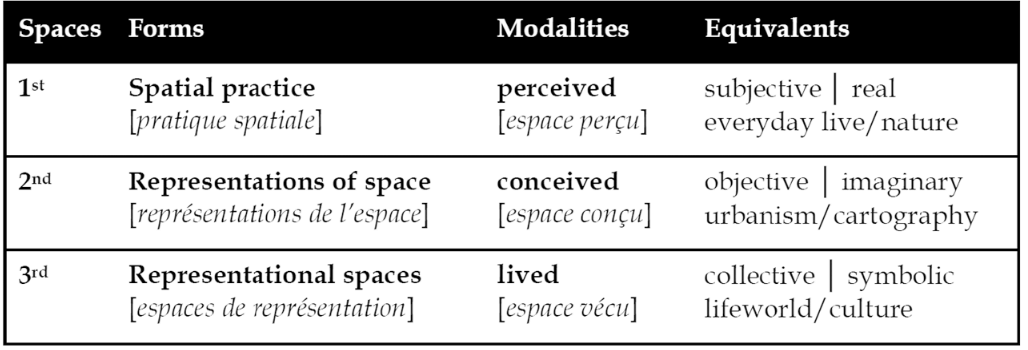
\includegraphics[width=\linewidth]{03-theory/lefebvretriad.png}
    \caption{Lefebvre's `Triad of Spaces' \citep[in][]{gunzel2019}}\label{fig: lefebvretriad}
\end{table}

Thus, de Certeau's distinction of space from place, whilst valuable insofar as it indicates the imbalance between human actors and institutions within the socio-cultural context - `the street, defined by urban planning is transformed into a space by walkers', in itself is hardly a novel realisation. Furthermore, its fecundity diminishes with the assertion that this relation should be understood solely through a linguistic lens, i.e. the rules of `place' are written by those with power, and `space' is the result of actions by participants reading and interpreting those rules. To view the relation as such is to say that the actions of participants must always lie within the diktat of place, and thus asserts that space originates in place and is therefore inseparable - `the only freedom you have is to formulate alternative sentences' \citep{vermeulen2015}. 

As Vermeulen further notes, for de Certeau, `space is an inter-subjective activation of a static site, a place', whilst for Lefebvre, `place is the momentary suspension of a social flow, [a] space'. This leads to a contradiction in the formulation of `agency' as a concept: `de Certeau understands agency as the enactment of a script not our own, whereas Lefebvre sees it not as a container for action but as the construction of action itself.' 

It's clear that with respect to \gls{4ec} approach to \textit{live} aesthetic experience it may be difficult to reconcile the 2nd and 3rd spaces of Lefebvre's triad (conceived and lived), due to its own anti-representationalist standpoint. However oppositional on that front however, Lefebvre's argument, through the prominence of social and class struggle under capitalism underpinning its formation, does indeed align itself with certain components (embodied, embedded) of enactivism: an approach that emphasises `the extended, intersubjective, and socially situated nature of cognitive systems' \citep[p. 6]{gallagher2017}: 
\begin{quote}
    `The relationship to space of a `subject' who is a member of a group or society implies a certain relationship to [their] body and vice versa.' \cite[p. 40]{lefebvre1991}
\end{quote}
Additionally, Lefebvre's `own particular brand of Marxism which stressed the importance of everyday life' \citep[p. 8]{merrifield1993} could be seen as aligned with Dewey's own assertion of the importance of artwork to return `origin and operation' in everyday experience. In this way, the construction of 2nd and 3rd space doesn't necessarily have to fall fully under the remit of \gls{4ec} to explicate in real-time or live experience, rather, they may constitute the socio-cultural, and environmental aspects (norms, values, laws, traditions, and conditions), as well as higher-order cognitive functions (meaning, and interpretation) that form the `environment', as it is then to be experienced \textit{or} later considered by the enactive cogniser.

Thus, whereas `the Metaverse' is somewhere to `show off your possessions', and `maybe even' stage social interaction \citep{marr2022}, augmented space in contrast, prioritises the social, cultural, and aesthetic experience of the everyday. Architecture in `the Metaverse', due to its origin in a capitalistic conception of society and technology, alienates its own inhabitants, since `under capitalism, it is only only through that [market] mediation that humans interact with buildings at all' \citep[p. 18]{mieville1998}. China Miéville's critique here of physical architecture under capitalism could also be applied to the profit motivation for the commodity fetishisation of art in \glspl{nft} and hence the Metaverse. Not just `virtual land', but digital art, music, video games, and social connection itself. More broadly, his `Marxist phenomenology' argues that to focus entirely on the physicality (of architecture in his text) is to `ignore the profound experiential ramifications' of living in a social system where such commodities are exchanged for profit. 

\begin{figure}[ht]
    \centering
    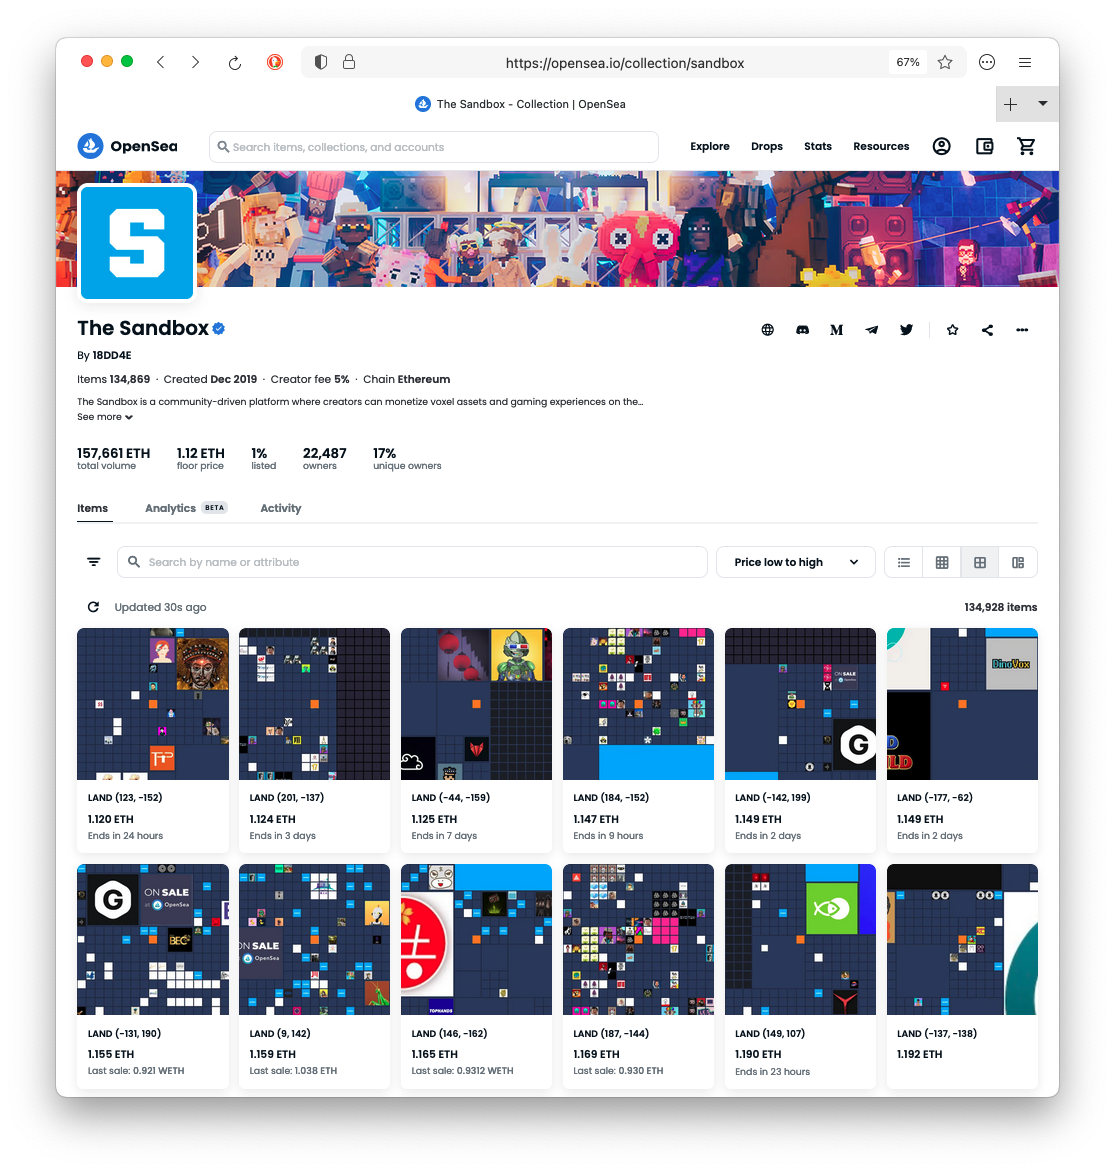
\includegraphics[width=.75\linewidth]{08-discussion/opensea2022_2.png}
    \captionsetup{justification=centering,margin=1.5cm}
    \caption{`Space' for sale in `The Metaverse' \citep[from][]{opensea2022}}\label{fig: opensea2022_2}
\end{figure}

In stark contrast, architecture in augmented space consists in a constantly unfolding dialogue between humans and their environment, as perceptually guided by an ecosystem of hybrid processes; rather than consisting in alienation, and the `anxiety' induced by the commodity fetishism underlying capitalist profit motives. Application of Lefebvrian spatial theory indicates that \gls{ar} can be a real force for social change, due to the way it can intervene spatially in the perception of participants, leading to new spatial characteristics and possibilities. When this is taken into action by people, either audiences, or performers, it puts the decision of when and where to `momentarily suspend' the social flow of space -- and thus construct `place' -- in their hands and in their bodies.

When Manifest.\gls{ar} virtually trespassed the \gls{moma} with invisible and intangible \gls{ar} art \citep{veenhof2010}; when \#OccupyAR broadcast the disembodied voices of geographically separated activists into Wall Street \citep{skwarek2018}; when Cem Kozar and Işıl Ünal \citeyearpar{thiel2011,thiel2018} revealed the unseen urban dynamics of the city of Istanbul, it was through the live co-construction of new hybrid spaces — augmented spaces — that once hidden realities could be enacted anew. Whilst one might see parallels between these actions and what de Certeau terms `tactics', the former, however, do more than just subverting place `proper' through `alternative sentences' to borrow Vermeulen's phrase. In actuality it is far more radical. Through the dynamic relations present in its hybridity — its incessant movement — emergent and novel states of self-organisation can occur within its constituents part(icipant)s. New socio-cultural meaning through sensory, perceptual and environmental modulation have the potential to synthesise from this ongoing process. In this momentary suspension of a social flow, `place' is co-constructed and enacted by the participants of the MoMA, Wall Street, and Istanbul. In the composition, experience, and performance of \textit{area\textasciitilde{}}, \textit{polaris\textasciitilde{}}, and \textit{polygons\textasciitilde{}} I glimpsed a part of this possibility.



